\documentclass[a4paper, 10pt]{article}
\usepackage[utf8x]{inputenc}
\usepackage[norsk]{babel}
\usepackage{natbib}
\usepackage{graphicx}
\usepackage[T1]{fontenc}
\usepackage{amsmath}
\usepackage{mathtools}
\usepackage{tabularx}
\usepackage{color, colortbl}
\usepackage{float}

\definecolor{Gray}{gray}{0.9}

\begin{document}
\begin{titlepage}
\begin{center} 

\vspace*{3cm}
\textsc{\Huge PU5}\\[0.7cm]
\textsc{\medium TTM4100 - Communication Services and Networks}\\[0.3cm]
\textsc{\medium TDT4140 - Software Enigneering}\\[0.3cm]
\textsc{\medium TDT4145 - Data Modeling, Databases and Database Management Systems}\\[0.3cm]
\textsc{\medium TDT4180 - Human-Computer Interaction}\\[0.3cm]

\textbf{\Large Gruppe 6:} \\[0.2cm]
\text{\Large Espen Albert, Finn Inderhaug, Kristoffer Andreas Dalby} \\
\text{\Large Christoffer B. Nysæter, Andreas Wien, Jonas André Dalseth}\\[1cm] 

\today

\end{center}
\end{titlepage}



\section{Use case}
\begin{figure}[h!] 
    \begin{center}  
        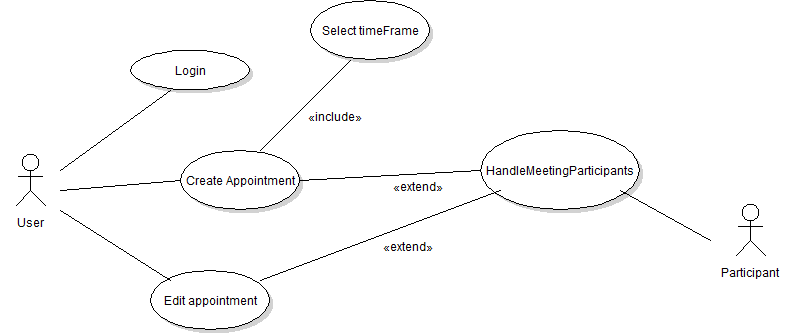
\includegraphics[width=8cm]{img/useCase1-4.png}
        \caption{class diagram}
    \label{class}
    \end{center}
\end{figure}


\section{Text use case}
\begin{tabularx}{\textwidth}{ |X|X| }
\hline
\rowcolor{Gray}
Use case &  Create appointment \\ \hline
Preconditions & Logged in \\ \hline
Steps & 
\begin{enumerate}
	\item User activates create appointment
	\item Title
	\item From time (date and time)
	\item To time (date and time)
	\item Optional: Location
	\item Optional: Description
	\item Optional: Select room
	\item Optional: Select participants
	\item Optional: Select groups
	\item Optional: Alarm
	\item Commit
\end{enumerate}\\ \hline
Expected result & 
\begin{enumerate}
	\item The appointment is created and shown in the calendar.
	\item All participants invited gets notified. 
\end{enumerate} \\ \hline
Possible errors & Users input a invalid value in from or to time. Reset from time and to time. \\ \hline


\end{tabularx}

\begin{tabularx}{\textwidth}{ |X|X| }
\hline
\rowcolor{Gray}
Use case &  Manage meeting participants \\ \hline
Preconditions & Logged in and appointment selected \\ \hline
Steps & 
\begin{enumerate}
	\item User activates create appointment
	\item Title
	\item From time (date and time)
	\item To time (date and time)
	\item Optional: Location
	\item Optional: Description
	\item Optional: Select room
	\item Optional: Select participants
	\item Optional: Select groups
	\item Optional: Alarm
	\item Commit
\end{enumerate}\\ \hline
Expected result & 
\begin{enumerate}
	\item The appointment is created and shown in the calendar.
	\item All participants invited gets notified. 
\end{enumerate} \\ \hline
Possible errors & Users input a invalid value in from or to time. Reset from time and to time. \\ \hline


\end{tabularx}


\begin{tabularx}{\textwidth}{ |X|X| }
\hline
\rowcolor{Gray}
Use case &  Edit appointment \\ \hline
Preconditions & Logged in and an appointment the user has created is selected \\ \hline
Steps & 
\begin{enumerate}
	\item User edits some of the fields in the appointment. (E.g. from time, end time, title, location, description, room)
	\item User clicks Commit
\end{enumerate}\\ \hline
Expected result & 
\begin{enumerate}
	\item The appointment is changed as expected. 
	\item The invited users get notified and can choose to accept or decline.
\end{enumerate} \\ \hline
Possible errors & 
\begin{scenario}
	\item Users input a invalid value in from or to time. >>Reset from time and to time.
	\item Users changes timeperiod, but the meeting room is occupied. >> Automatically assign a new meeting room for the user.
\end{scenario} \\ \hline
\end{tabularx}

\newpage

\section{Sequence diagram}
\begin{figure}[h!] 
    \begin{center}  
        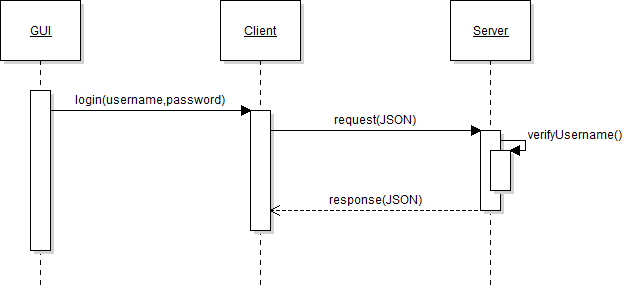
\includegraphics[width=8cm]{img/seqLogin.png}
        \caption{class diagram}
    \label{class}
    \end{center}
\end{figure}

\begin{figure}[h!] 
    \begin{center}  
        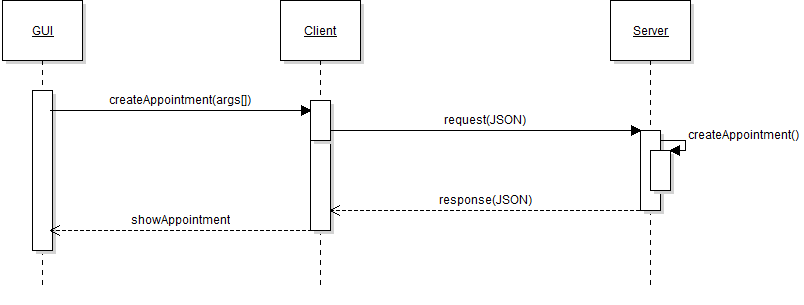
\includegraphics[width=8cm]{img/seqCreateAppointment.png}
        \caption{class diagram}
    \label{class}
    \end{center}
\end{figure}

\begin{figure}[h!] 
    \begin{center}  
        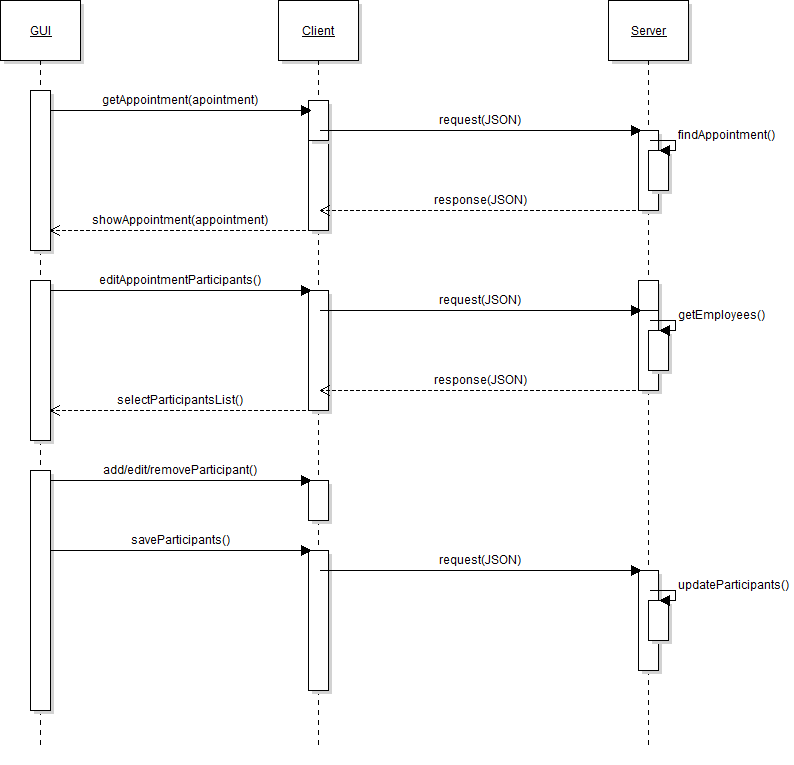
\includegraphics[width=8cm]{img/seqManageParticipants.png}
        \caption{class diagram}
    \label{class}
    \end{center}
\end{figure}

\begin{figure}[h!] 
    \begin{center}  
        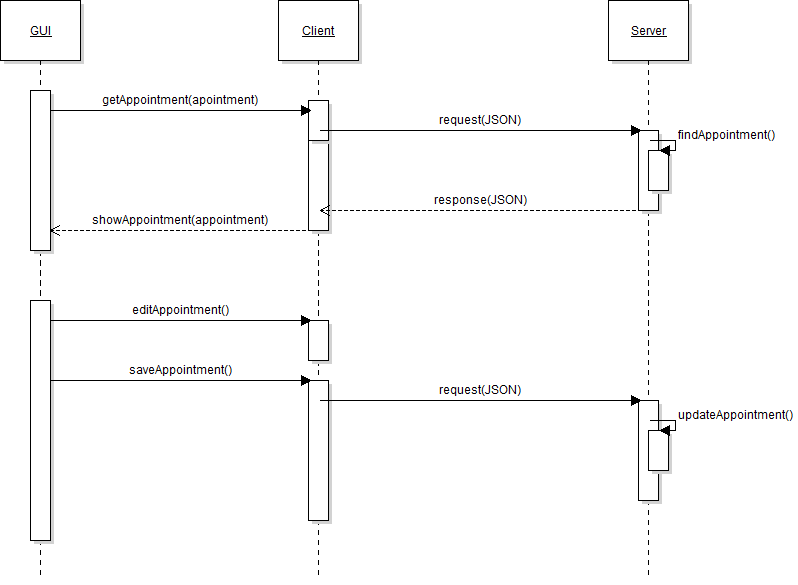
\includegraphics[width=8cm]{img/seqEditAppointment.png}
        \caption{class diagram}
    \label{class}
    \end{center}
\end{figure}

\newpage

\section{System structure}
The system will be implemented in a server/client configuration where each user need their own client on their own computer and the server is hosted on its own computer. The server-side is the only piece of the software that interacts with the database. All the information from every client is saved in the database. Between the client and the server, the information is sent formatted as JSON. The frontend will be written in Java Swing.

\subsubsection{User}
The User class is one of the more important classes in the system, it defines the way our users are handled. Every user will have a username, password, name and email. They also have a list of alarms that is related to the user.

\subsubsection{Appointment}
The Appointment class is where we implement how every appointment is handled. An appointment has a id, title, description, timeframe, owner, participants and room/location. The room/location is mainly based on the need for a meeting room.

\subsubsection{MeetingRoom}
The MeetingRoom class is where we handle the meeting rooms. It is a basic class which only holds information about id, room, capacity and reservations.

\subsubsection{Group}
Group is a class what collects users in groups, it only contains an id, groupname and a list of users.

\subsubsection{Alarm}
Alarm is a little class that holds the date and time information about when a alarm should be executed.

\subsubsection{TimeFrame}
TimeFrame is a class that holds the duration of time. It has a startdate and an enddate, it can provide the duration of itself. It is mainly used to set time for appointments and reserve meeting rooms.



\end{document}
